\section{Information about some enttity(s)}
\label{sec-information-about}

\textbf{Created by:} Arkopaul Sarkar \\
\textbf{Modified by:}

\subsection*{Scenario Objective}
This scenario illustrates how various types of information about an entity (e.g., object, process, properties) can be captured. This scenario introduces the fundamental classes and properties to model information. Although IOF contains many types of informational entities, this scenario only introduces the generic types of information based on how they refer to the entities they are about.  

\subsection*{General Pattern Description}

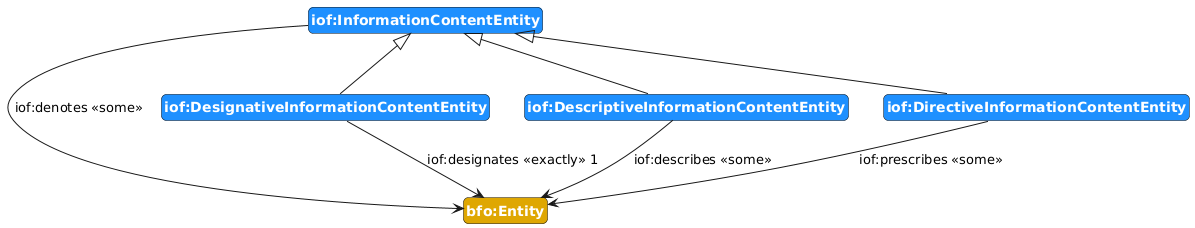
\includegraphics[scale=0.4]{scenarios/information-and-aboutness/images/general-information-aboutness.png}

The primitive and generic relationship \texttt{iof:isAbout} establishes a connection between an Information Content Entity (ICE) and a referenced entity, encapsulating the fundamental notion of ``aboutness''—that is, the ICE instance conveys information about the entity.

Three distinct modes of referring to an entity are captured through three specialized sub-properties of \texttt{iof:isAbout}: \texttt{iof:denotes} serves to distinguish one or more instances of an entity.
\texttt{iof:designates}, a functional specialization of \texttt{iof:denotes}, uniquely identifies a single specific instance, ensuring exclusive reference.
\texttt{iof:describes} conveys attributes or characteristics of an entity without necessarily providing unique identification. It emphasizes detailing the entity rather than establishing a direct referential link.
\texttt{iof:prescribes} refers to entities that may not yet exist but are expected to adhere to prescribed rules, guidelines, or specifications once instantiated. It thus encompasses potential future entities, such as artifacts constructed according to a design specification or processes executed in alignment with a plan specification.
Accordingly, the IOF Core ontology defines three corresponding classes of ICE—Designative ICE, Descriptive ICE, and Prescriptive ICE—each characterized based on these three sub-properties of \texttt{iof:isAbout}. 

\subsection*{Use Case Pattern Description}

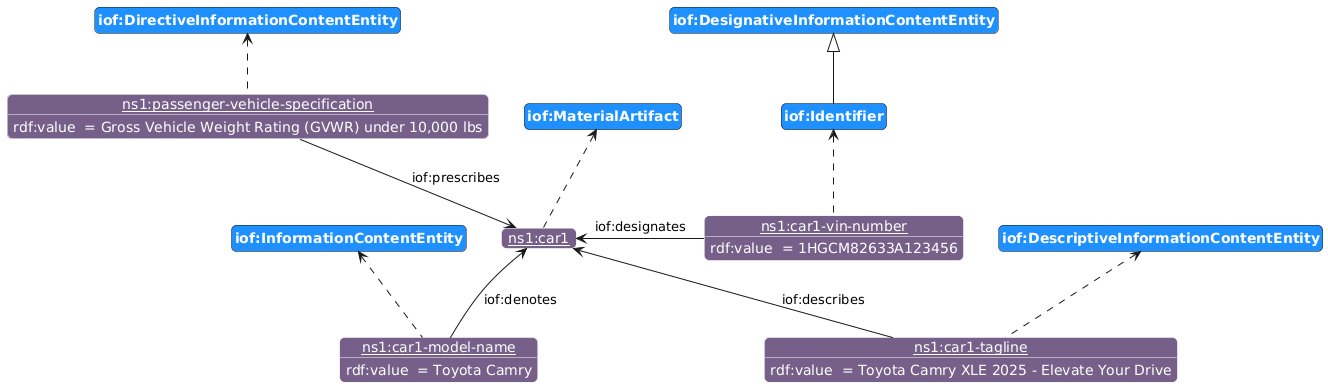
\includegraphics[scale=0.5]{scenarios/information-and-aboutness/images/uc1-ices.png}


\subsubsection*{Use-Case Example Data}


\subsubsection*{Data Mapping}


\subsubsection*{Data Validation}
